\subsection{M-WEM Simulations of Alanine Dipeptide}

\subsubsection{Introduction}

The Markovian Weighted Ensemble Milestoning (M-WEM) approach \citep{Ray2022Markovian} is a modified version of the Weighted Ensemble Milestoning (WEM) \citep{Ray2020Kinetics,Ray2020Weighted} approach. 
Both approaches are designed to use the WE strategy to enhance the efficiency of the milestoning method in calculating equilibrium and non-equilibrium properties (e.g., free energy landscape and rate constants, respectively). 

In the milestoning method \citep{Faradjian2004Computing,West2007Extending} the reaction coordinate is stratified using multiple high-dimensional interfaces---or milestones. 
Short trajectories are propagated between the interfaces and using the principles of continuous time Markov chains, the properties of a long timescale process can be calculated. 
But the milestones need to be placed significantly far from each other to lose memory of the previous milestone. 
But converging the transition statistics between distant milestones can be expensive depending on the underlying free energy landscape and the complexity of the system. 
Because of the use of shorter trajectories that do not require trajectories to transit from the initial to final states, the WEM and M-WEM calculations are computationally less expensive than a WE simulation. 
On the downside, however, one cannot obtain continuous pathways due to the lack of continuous trajectories between the starting and the final state. 

In the M-WEM approach, regions between the milestones are referred to as “cells”.
WE simulation is performed within the cell with half-harmonic walls present at the milestone interfaces to prevent trajectory escape \citep{Vanden-Eijnden2009Markovian, Maragliano2009Free, Ray2022Markovian}. 
In this tutorial, we will use M-WEM to calculate the mean first passage time (MFPT), free energy landscape and committor function for the conformational transition in the alanine dipeptide system.

\textbf{Learning objectives.} This tutorial covers the installation of and use of the Markovian Weighted Ensemble Milestoning (M-WEM) software in combination with WESTPA to compute the kinetics and the free energy landscape of an alanine dipeptide. 
Specific learning objectives include:

\begin{enumerate}
  \item How to install the M-WEM software and perform an M-WEM simulation;
  \item How to create milestones to define the M-WEM progress coordinate;
  \item How to analyze an M-WEM simulation to compute the mean first passage time, committor, and free energy landscape. 
\end{enumerate}

\subsubsection{Prerequisites}

The users should have a basic understanding of running WE simulations using the Minimal Adaptive Binning (MAB) scheme, and should have completed \textbf{Advanced Tutorial 3.2} before commencing the M-WEM tutorial. 
Also, a basic idea of the Markovian Milestoning framework is necessary. 
For that purpose, the users should refer to the following manuscripts \cite{Vanden-Eijnden2009Markovian, Maragliano2009Free, Ray2022Markovian}.

\textbf{Computational requirements.} In terms of software, this tutorial requires several Python modules (Numpy, Scipy, and Matplotlib) in addition to the WESTPA 2.0 software and NAMD 2.14 simulation package. 
Note: M-WEM is implemented using the colvars module in NAMD. 
Please check out the NAMD tutorial ({\url{http://www.ks.uiuc.edu/Training/Tutorials/namd-index.html}}) and colvars tutorial ({\url{https://colvars.github.io/colvars-refman-namd/colvars-refman-namd.html}}).
 
In terms of computer hardware, this tutorial will require approximately 4 GB of disk space. 
Running the simulation 100 WE iterations for each milestone takes \textasciitilde85 min on an Intel Core i5-8250U CPU @ 1.60GHz processor with 4 CPU cores. 
For 8 milestones that amounts to about 11-12 hr if the calculation is performed serially with 4 CPU cores used at a time. 
But if a computer cluster is available, each milestone should be run in parallel which will significantly reduce the wall clock time. 
The analysis for each milestone takes \textasciitilde5 min for each milestone with the same computing hardware but with 1 CPU core. 
For 8 milestone cells that would be \textasciitilde40 min, but similar to the simulation, the analysis for each milestone can be done in parallel.  

\subsubsection{Installation of the M-WEM software package}

The \verb|M-WEM| software package can be downloaded from {\url{https://github.com/dhimanray/MWEM}}. 
To install the package go to the main directory that contains the \verb|setup.py| file and run the following command:

\begin{verbatim}
  $ python -m pip install .
\end{verbatim}

The M-WEM software should be installed in the same conda environment in which WESTPA 2.0 is installed.

\subsubsection{Setting up a M-WEM environment}

\textbf{Overview.} For performing the M-WEM simulation, we need to first create the milestone anchors along the transition pathway. 
This is a typical prerequisite for milestoning simulation. 
It is typically done using steered MD simulation \citep{griebel_steered_1999} which is a common technique in MD simulation. 
To avoid spending extra time and possible variability in the results, we have generated the milestone anchors and provided them in the anchors directory.

% for single column figure don't include the *
\begin{figure}[t]
\centering
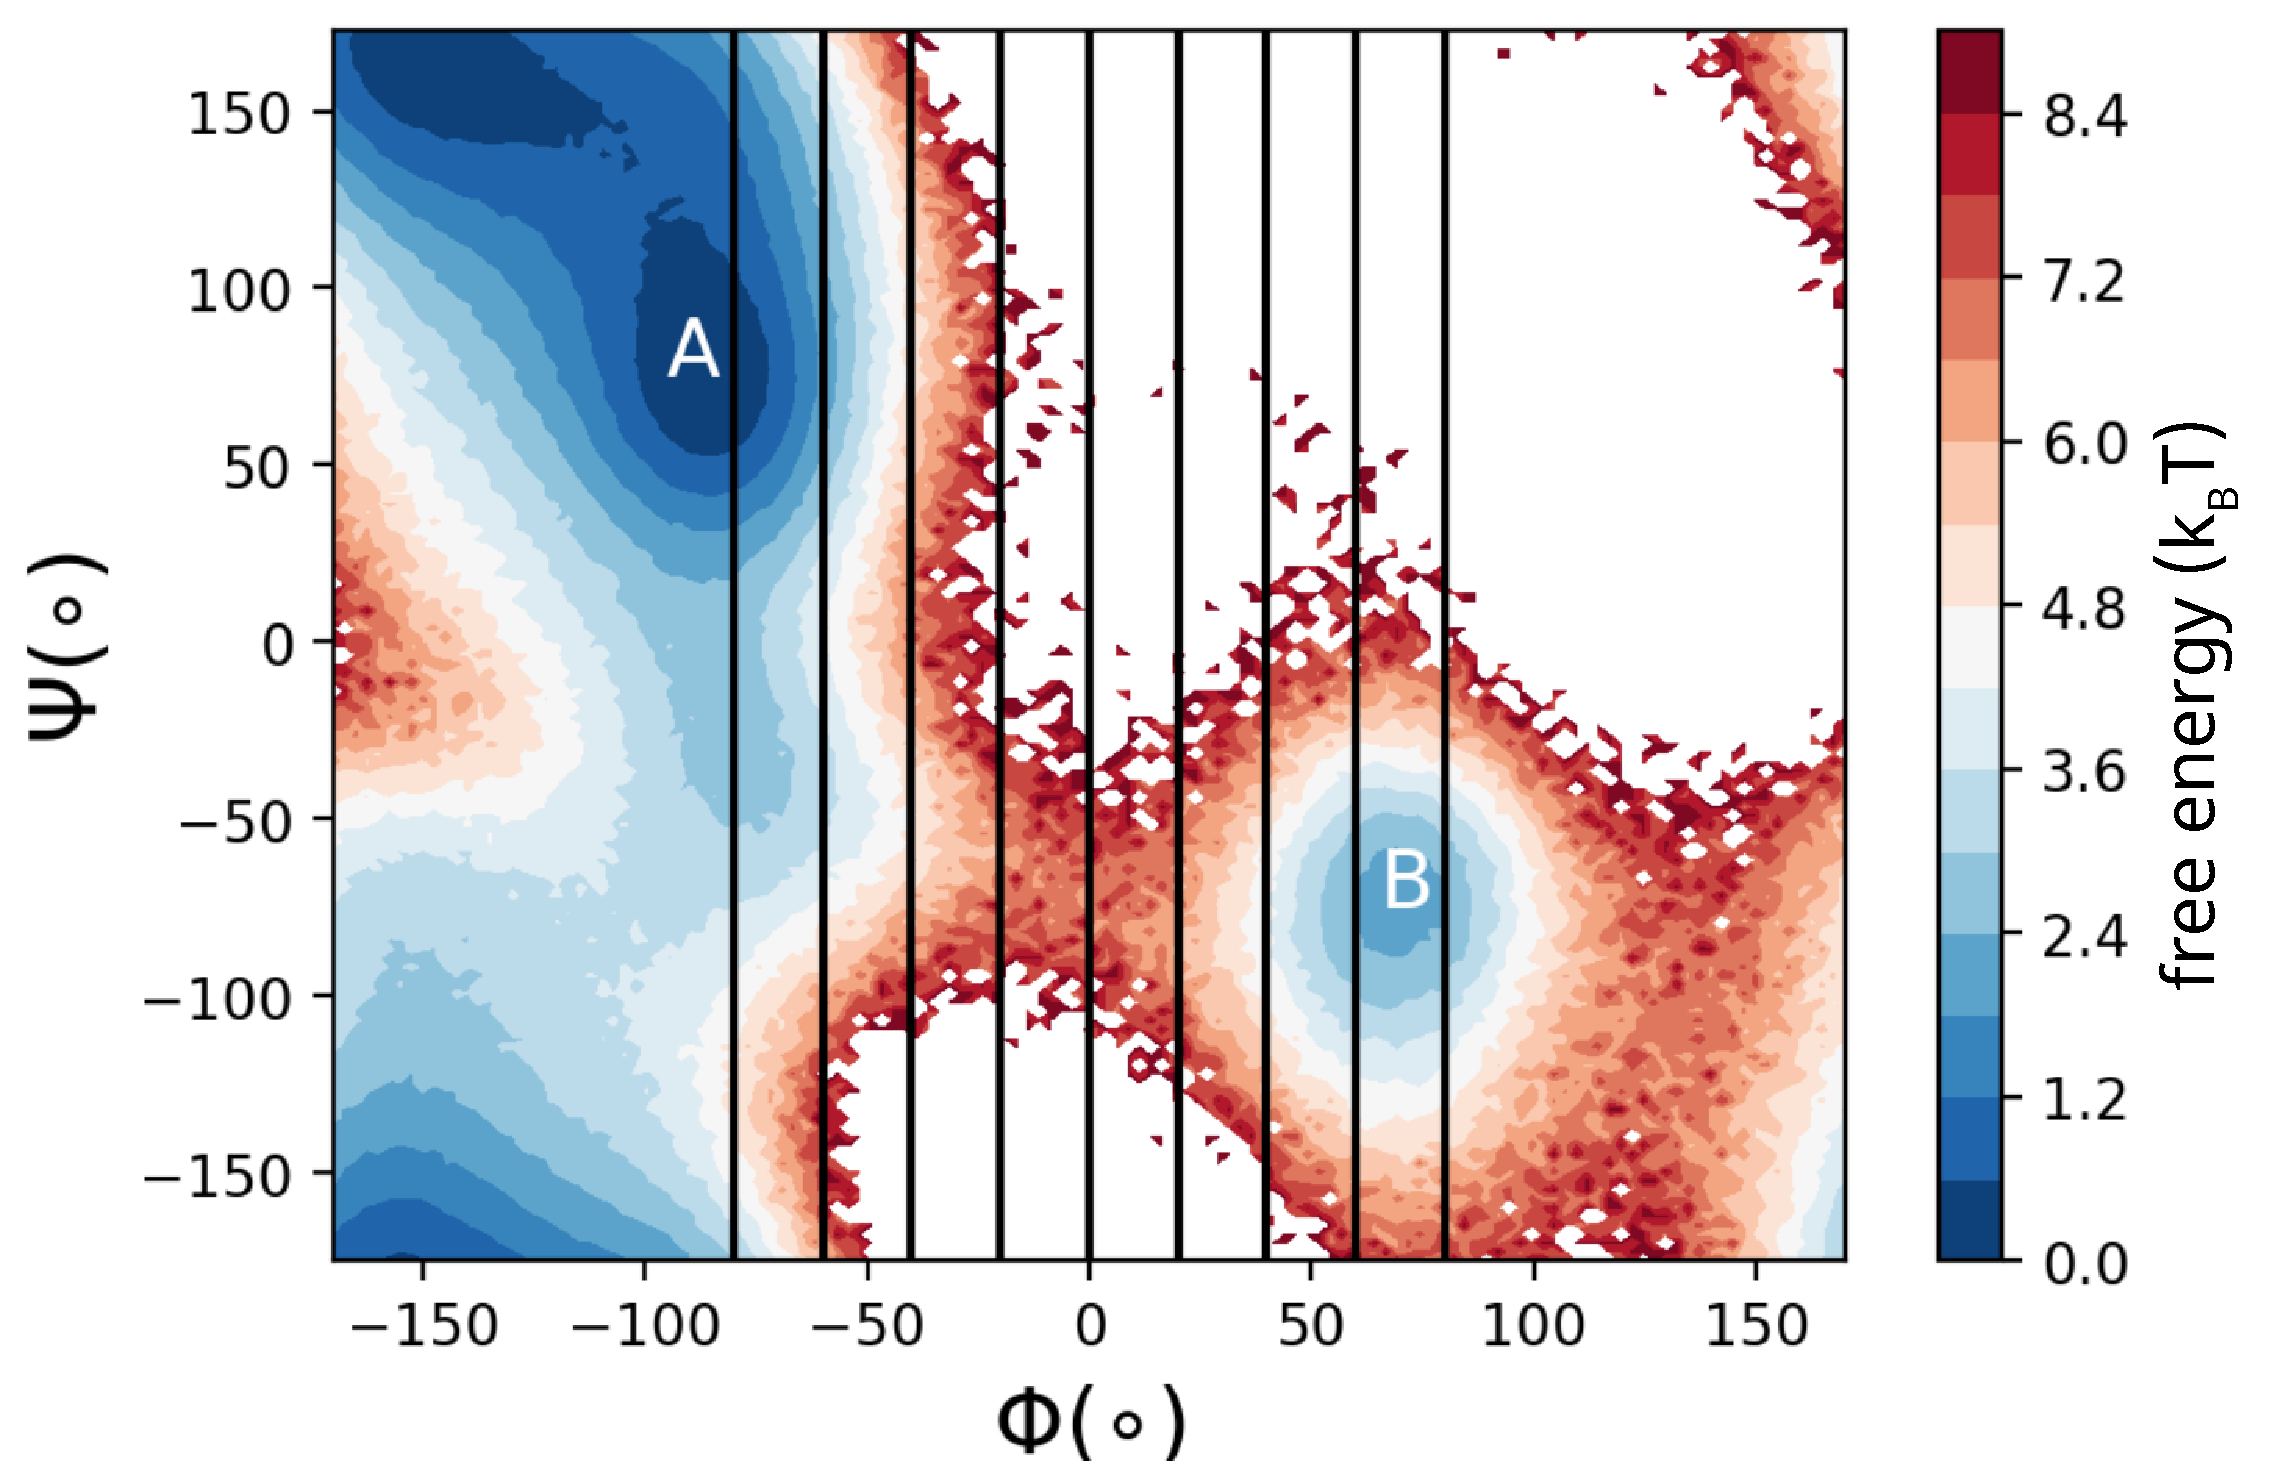
\includegraphics[width=\columnwidth]{figures/Figure9_RBin.pdf}
\caption{Free energy landscape of alanine dipeptide in the gas phase. Milestone positions are shown as vertical lines. 
Our aim is to simulate the MFPT of the transition from state A to state B.}
\end{figure}

\textbf{The system.} We will be studying the conformational change of gas phase alanine dipeptide using the M-WEM scheme. 
The details of this example are provided in the article: Ray et al. 2022 \citep{Ray2022Markovian}. 

The free energy landscape for the system is shown in \textbf{Figure 9}. 
To simulate the transition from state A to state B, 9 milestones are placed at $\phi$ = -80$^{\circ}$,  -60$^{\circ}$, -40$^{\circ}$, -20$^{\circ}$, 0$^{\circ}$, 20$^{\circ}$, 40$^{\circ}$, 60$^{\circ}$, 80$^{\circ}$. 
This created 8 cells bound by the milestones. 
The anchors are chosen in a way that they are located approximately in the middle of each cell.

\textbf{Preparing the simulation environment.} The \verb|tutorial-3.5/| directory contains all simulation and analysis files and will be referred to as the simulation home directory for the rest of the tutorial. 
The milestone anchors for all cells generated from the steered MD simulation are provided as pdb files in the \verb|anchors/| directory. 

The \verb|build.py| script is a python script which will set up all the milestones for the simulation. 
Each milestone cell will be simulated in a different directory, numbered from 0 to 7. 

The \verb|template/| directory is a generic template for M-WEM simulation for any one cell. 
It contains all necessary files except for the pdb files which are specific to each cell (which are in the \verb|anchors/| directory). 
Also, the \verb|colvars.in| files have replaceable strings which are used by the \verb|build.py| script to create cell specific files. 
For example, there are terms like "CENTER", "HIGH", and "LOW". These are places where the position of the center and the two milestones are written by the \verb|build.py| code. 
Make sure to edit the \verb|env.sh| file to include the path to your NAMD installation.

In the \verb|common_files/| directory the topology (.psf), the parameter (.prm) and the NAMD configuration files are provided. 
The structure file (.pdb) in this directory and in the \verb|equilibration/| directory are prepared by the \verb|build.py| script, and are different for each milestone cell. 

Once you have your M-WEM setup ready, prepare the cell-specific folders by running the following command:

\begin{verbatim}
  $ python build.py
\end{verbatim}

\subsubsection{Running the M-WEM simulation} In the \verb|equilibration/| directory of each cell, a constrained equilibration of the anchor will need to be performed to keep the anchor approximately in the middle of the cell. 
The \verb|milestone_equilibration.colvars.traj| file contains the collective variable information, which, in this case, are the Phi and Psi torsion angles of the alanine dipeptide. 
The \verb|milestone_equilibration.xsc|, \verb|milestone_equilibration.coor| and\linebreak \verb|milestone_equilibration.vel| files are NAMD restart files that will be used to start WE trajectories from the endpoint of the equilibration simulation. 

The running of the M-WEM simulation for each individual cell is done separately, for the convenience of parallelizing it in a computing cluster. 
The \verb|run.sh| script performs the simulation via the command \verb|./run.sh|.
Unlike typical WESTPA setups, here the initialization setup code is included in the \verb|run.sh| script. 
Although it does not make a significant difference for a small system like this, we found it is more convenient to submit multiple milestone jobs to a computer cluster by using a single \verb|run.sh| script. 
Both the equilibration and running of each cell is performed by executing the following command from within each cell-specific folder:

\begin{verbatim}
  $ ./run.sh
\end{verbatim}

In the first part of the script, equilibration is performed. 
Then relevant files are copied to the \verb|bstates/| directory, from which they are read by the \verb|westpa_scripts/runseg.sh|. 
Then the WE simulation is initialized and propagated as usual by the \verb|w_init| and \verb|w_run| commands. 
In this example script, only one trajectory is propagated at a time. 
But this can be parallelized based on the computing resources available.
Alternative Slurm scripts for running and restarting the simulation are also provided in the same directory.

The total number of iterations performed per milestone is 100. 
The user may choose to change this number according to their preference. 
The results reported in this work are from 100 iterations. 
The convergence is achieved after 40 iterations in our calculation. 
But it may slightly vary for independent calculations.

\subsubsection{Analyzing the M-WEM simulations} After the M-WEM simulations are completed, it is important to properly analyze the results. 
Please refer to the M-WEM publication for the theoretical details of the analysis \cite{Ray2022Markovian}. 
We perform the analysis in two steps:

\textbf{Step 1.} Move into the \verb|analysis/| directory and execute the following command: 

\begin{verbatim}
  $ python analysis_build.py 
\end{verbatim}

The \verb|analysis_build.py| script will produce directories \verb|cell_0/| through \verb|cell_7/| and copy the corresponding \verb|west.h5| files (WESTPA output files) from the \verb|propagation/| directory into each cell. 
It will also copy the \verb|west.cfg| files (different from the \verb|west.cfg| files for propagation), and the \verb|analysis.py| files from \verb|westpa_analysis_files/| directory to each cell. 
The \verb|analysis.py| file also has strings like "LOW" and "HIGH", which will be replaced by floating point numbers corresponding to the left and right milestones.

Running the \verb|analysis.py| script from within a specific cell directory will produce the \verb|trajectories.pkl|, \verb|crossings.pkl| and \verb|weights.txt| files. 
The files generated by \verb|analysis.py| contain information on the trajectory traces (history of the segments in the final iteration), the time and location (which milestone right or left) of the milestone crossings, and the weights of each traced trajectory respectively.

% for single column figure don't include the *
\begin{figure}[t]
\centering
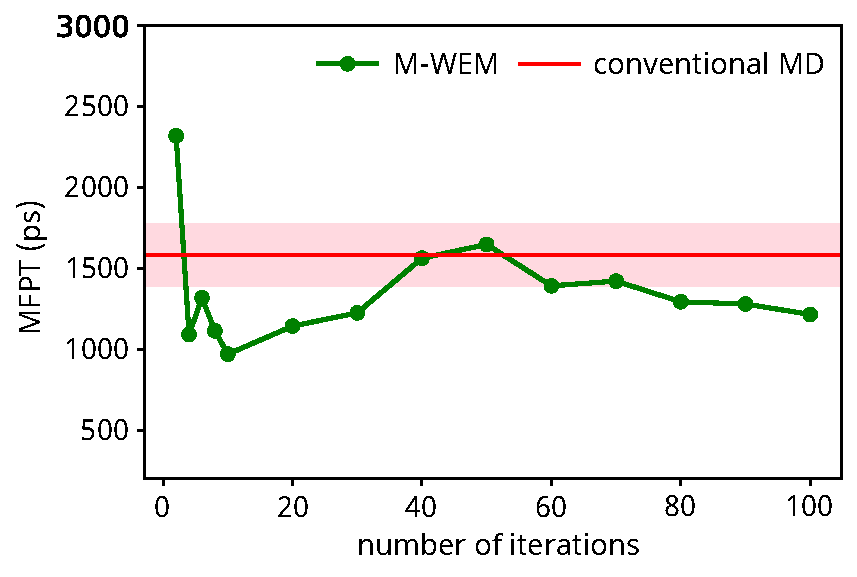
\includegraphics[width=\columnwidth]{figures/Figure10_MFPT.pdf}
\caption{Convergence of the mean first passage time (MFPT) as a function of M-WEM iterations.}
\end{figure}

% for single column figure don't include the *
\begin{figure}[t]
\centering
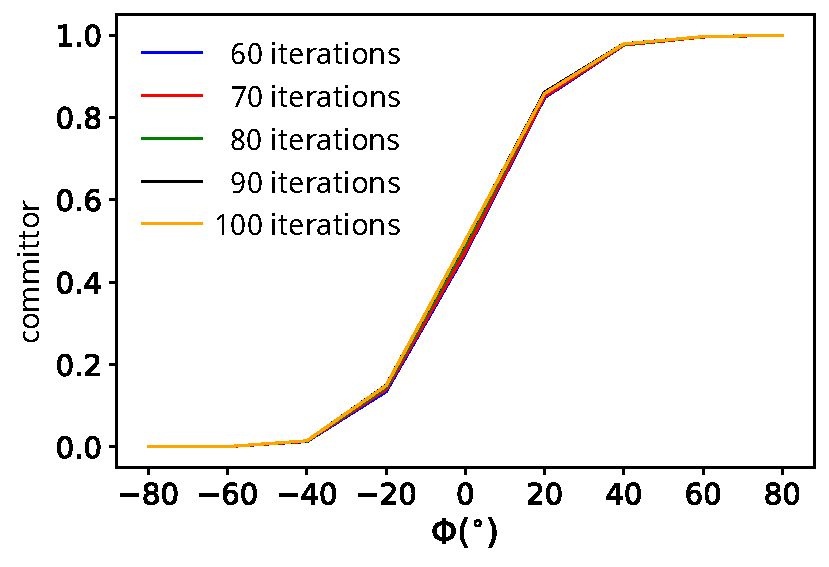
\includegraphics[width=\columnwidth]{figures/Figure11_Committor.pdf}
\caption{Committor function along the $\phi$ coordinate from M-WEM simulation.}
\end{figure}

Perform analysis in all cells by running the following command from within the \verb|analysis/| directory:

\begin{verbatim}
  $ ./analyze_all_convergence.sh
\end{verbatim}

This script will execute \verb|python analysis.py| from within each cell-specific directory to produce the .pkl and .txt outputs for the final iteration. 
But, for the sake of checking convergence of our results, it will also produce similar files for some subsequent iterations. 
To do that, the script will copy the \verb|analysis.py| to \verb|analysis_x.py| (where x = iteration number) and replace the \verb|w.niters| inside each \verb|analysis.py| to the corresponding iteration number. 
Then, it will produce \verb|trajectories_x.pkl|, \verb|crossings_x.pkl| and the \verb|weights_x.txt| files for each x. 
This step can take several minutes to a few hours depending on the computing hardware. 
If you have access to a computing cluster, you may choose to submit this as a job.
Note that the \verb|analyze_all_convergence.sh| script is customizable. 
For example, if you want to run all cells in parallel on a cluster you can create separate bash scripts for each cell. 
Also, \verb|analysis_build.py| will produce the following directories for milestoning analysis in Step 2: \verb|cell_probability/|, \verb|N_i_j_files/|, \verb|R_i_files/|, and \verb|committor/|.

\textbf{Step 2.} After the analysis of the WESTPA output files are done, we will proceed to analyze our results using the Markovian milestoning framework in two Jupyter notebooks: \verb|kinetics.ipynb| and \verb|free-energy-landscape.ipynb|.

First run the \verb|kinetics.ipynb| notebook to obtain the mean first passage time and the committors. 
This will also produce the probability distribution file in the milestone space. Details can be found inside the notebook. 
The MFPT convergence plots and the committor functions should look like \textbf{Figures 10 and 11}.

% for single column figure don't include the *
\begin{figure}[t]
\centering
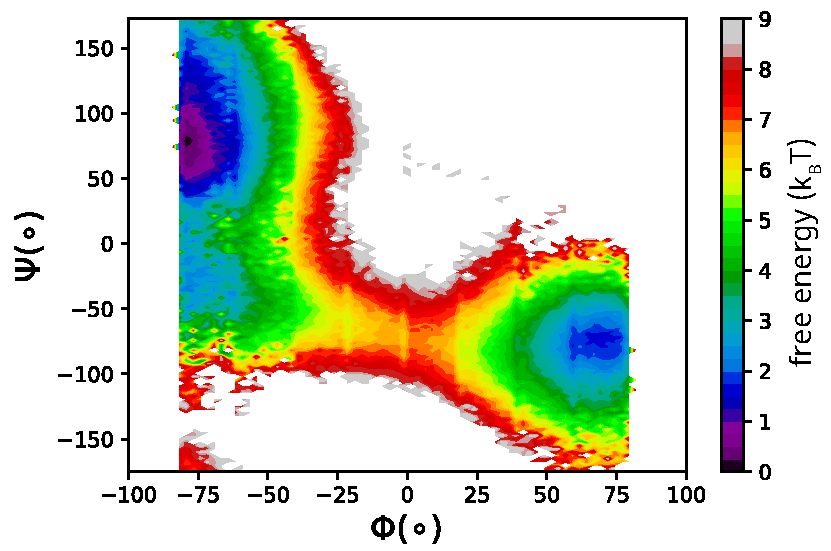
\includegraphics[width=\columnwidth]{figures/Figure12_RFree.pdf}
\caption{Free energy landscape reconstructed from an M-WEM simulation.}
\end{figure}

Next, run the \verb|free-energy-landscape.ipynb| to reconstruct the free energy landscape along Phi and Psi coordinates from the M-WEM data. 
It will first produce the unscaled probability distribution, rescale it and then compute the rescaled free energy landscape. 
The final free energy landscape should look like \textbf{Figure 12}.

Note that before executing any notebook, you will need to set the kernel to the environment in which you installed the M-WEM software. 
If the kernel is not available, activate the Jupyter notebook for that environment by executing:

\begin{verbatim}
  $ python -m ipykernel install --user --name=westpa2
\end{verbatim}
Replace westpa2 with the environment in which you installed M-WEM.

\subsubsection{Conclusion}
This tutorial presents the Markovian Weighted Ensemble Milestoning (M-WEM) Python package for use with the WESTPA 2.0 software package to estimate equilibrium and non-equilibrium observables for the alanine dipeptide. 
In the M-WEM approach, the WE strategy is applied to enhance the efficiency of the Markovian milestoning approach to accelerate the convergence between milestones.
While it is not possible to use this approach to generate continuous pathways between the initial and final states of a rare-event process, the M-WEM approach can be highly efficient in the calculation of  “end-point properties” such as the MFPT and free energy differences between the two states. 
Beyond the alanine dipeptide, the M-WEM approach has been applied to more complex processes such as receptor-ligand binding, yielding the $k_{on}$, $k_{off}$, and binding free energy for the trypsin benzamidine complex \citep{Ray2022Markovian}.